% begin module limits-ex7
\begin{frame}
By comparing the definitions, we can see that
\[
\lim_{x\rightarrow a} f(x) = L \ \text{ if and only if } \lim_{x\rightarrow a^-}f(x) = L \ \text{ and } \lim_{x\rightarrow a^+}f(x) = L .
\]
\begin{example}[Example 7, p. 100]
\begin{columns}[c]
\column{.55\textwidth}
The graph of a function $g$ is shown to the right.  Use it to state the values (if they exist) of the following:
\begin{align*}
\alert<handout:0| 2-3>{\lim_{x\rightarrow 1^-}g(x)} & \alert<handout:0 |2-3>{=} \alert<handout:0 |3>{\uncover<3->{3}} &%
\alert<handout:0| 8-9>{\lim_{x\rightarrow 3^-}g(x)} & \alert<handout:0 |8-9>{=} \alert<handout:0 |9>{\uncover<9->{1}} \\%
\alert<handout:0| 4-5>{\lim_{x\rightarrow 1^+}g(x)} & \alert<handout:0 |4-5>{=} \alert<handout:0 |5>{\uncover<5->{3}} &%
\alert<handout:0| 10-11>{\lim_{x\rightarrow 3^+}g(x)} & \alert<handout:0 |10-11>{=} \alert<handout:0 |11>{\uncover<11->{2}} \\%
\alert<handout:0| 6-7>{\lim_{x\rightarrow 1}g(x)} & \alert<handout:0 |6-7>{=} \alert<handout:0 |7>{\uncover<7->{3}} &%
\alert<handout:0| 12-13>{\lim_{x\rightarrow 3}g(x)} & \alert<handout:0 |12-13>{=} %
 \uncover<13->{\alert<handout:0| 13>{\text{DNE}}} %
\end{align*}
\column{.45\textwidth}
 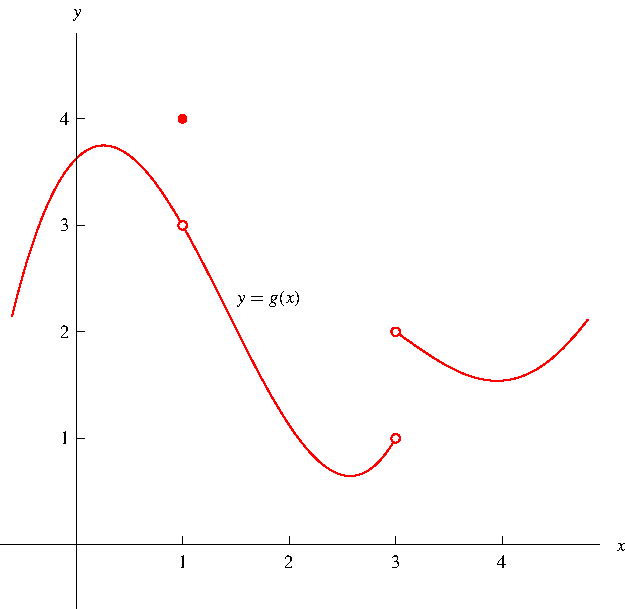
\includegraphics[height=5cm]{limits/pictures/02-02-ex7.pdf}%
\end{columns}
\end{example}
\end{frame}
% end module limits-ex7
